\documentclass{beamer}

\mode<presentation>{
    \usetheme{Madrid}
    \usecolortheme{dolphin}
}
\usepackage{graphicx}
\usepackage{booktabs}
\usepackage{amsmath}
\usepackage{amssymb}
\usepackage{tabularx}
\usepackage[utf8]{inputenc}
\usepackage[english]{babel}
\usepackage{hyperref}
% \usepackage{listings}
\title[Big Data Methods for Economists]{Support Vector Machines}
\author{
    Wenjie Tu \\
}
\institute[UZH]{
    University of Zurich \\
    \medskip
    \textit{\href{wenjie.tu@uzh.ch}{wenjie.tu@uzh.ch}} \\
}
\date{March 26, 2021}

\begin{document}

\begin{frame}
\titlepage 
\end{frame}

\begin{frame}
    \frametitle{Overview}
    \tableofcontents
\end{frame}
    
\section{Maximal Margin Classifier}
\subsection{Classification Using the Separating Hyperplane}
\subsection{Classification Using the Maximal Margin Classifier}
\subsection{Construction of the Maximal Margin Classifier}
\subsection{The Non-separable Case}

\section{Support Vector Classifiers}
\subsection{Overview of the Support Vector Classifier}
\subsection{Classification Using the Support Vector Classifier}

\section{Support Vector Machines}
\subsection{Classification with Non-linear Decision Boundaries}
\subsection{The Support Vector Machine}

\section{SVMs with More than Two Classes}
\subsection{One-Versus-One Classification}
\subsection{One-Versus-All Classification}

% \section{Applications in R}

\begin{frame}
    \frametitle{Maximal Margin Classifier}
    \framesubtitle{Classification Using a Separating Hyperplane}
    \begin{block}{Hyperplane}
        In a $p$-dimensional space, a \textit{hyperplane} is a flat affine subspace 
        of dimension $p-1$.
    \end{block}

    \begin{block}{Exmaples}
        \begin{itemize}
            \item In two dimensions, a hyperplane is defined by 
            \[\beta_0 + \beta_1 X_1 + \beta_2 X_2 =0 \] 
            \item In $p$ dimensions, a hyperplane is defined by 
            \[\beta_0+\beta_1 X_1 + \beta_2 X_2 + \cdots +\beta_pX_p=0 \] 
        \end{itemize}
    \end{block}
\end{frame}



\begin{frame}
    \frametitle{Maximal Margin Classifier}
    \framesubtitle{Classification Using a Separating Hyperplane}
    Suppose that there exists a point $X=(X_1,X_2,\cdots,X_p)^T$ in the $p$ dimensional space
    \begin{itemize}
        \item If $X$ satisifes $\beta_0+\beta_1 X_1 + \beta_2 X_2 + \cdots +\beta_pX_p=0$, 
        then $X$ lies on the hyperplane.
        \item If $X$ satisfies $\beta_0+\beta_1 X_1 + \beta_2 X_2 + \cdots +\beta_pX_p>0$, 
        then $X$ lies on the one side of the hyperplane.
        \item If $X$ satisfies $\beta_0+\beta_1 X_1 + \beta_2 X_2 + \cdots +\beta_pX_p<0$, 
        then $X$ lies on the other side of the hyperplane.
    \end{itemize}
\end{frame}



\begin{frame}
    \frametitle{Maximal Margin Classifier}
    \framesubtitle{Classification Using a Separating Hyperplane}
    In binary classification, we can label the observations from one class as $y_i=1$ 
    and those from the other class as $y_i=-1$.
    \begin{align*}
        \begin{cases}
            \beta_0+\beta_1x_{i1}+\beta_2x_{i2}+\cdots+\beta_px_{ip}>0 & y_i=1 \\
            \beta_0+\beta_1x_{i1}+\beta_2x_{i2}+\cdots+\beta_px_{ip}<0 & y_i=-1
        \end{cases}
\end{align*}

Equivalently,
\[y_i(\beta_0+\beta_1x_{i1}+\beta_2x_{i2}+\cdots+\beta_px_{ip})>0 \] 
\end{frame}





\begin{frame}
    \frametitle{Maximal Margin Classifier}
    \framesubtitle{Classification Using a Separating Hyperplane}

    \begin{center}
        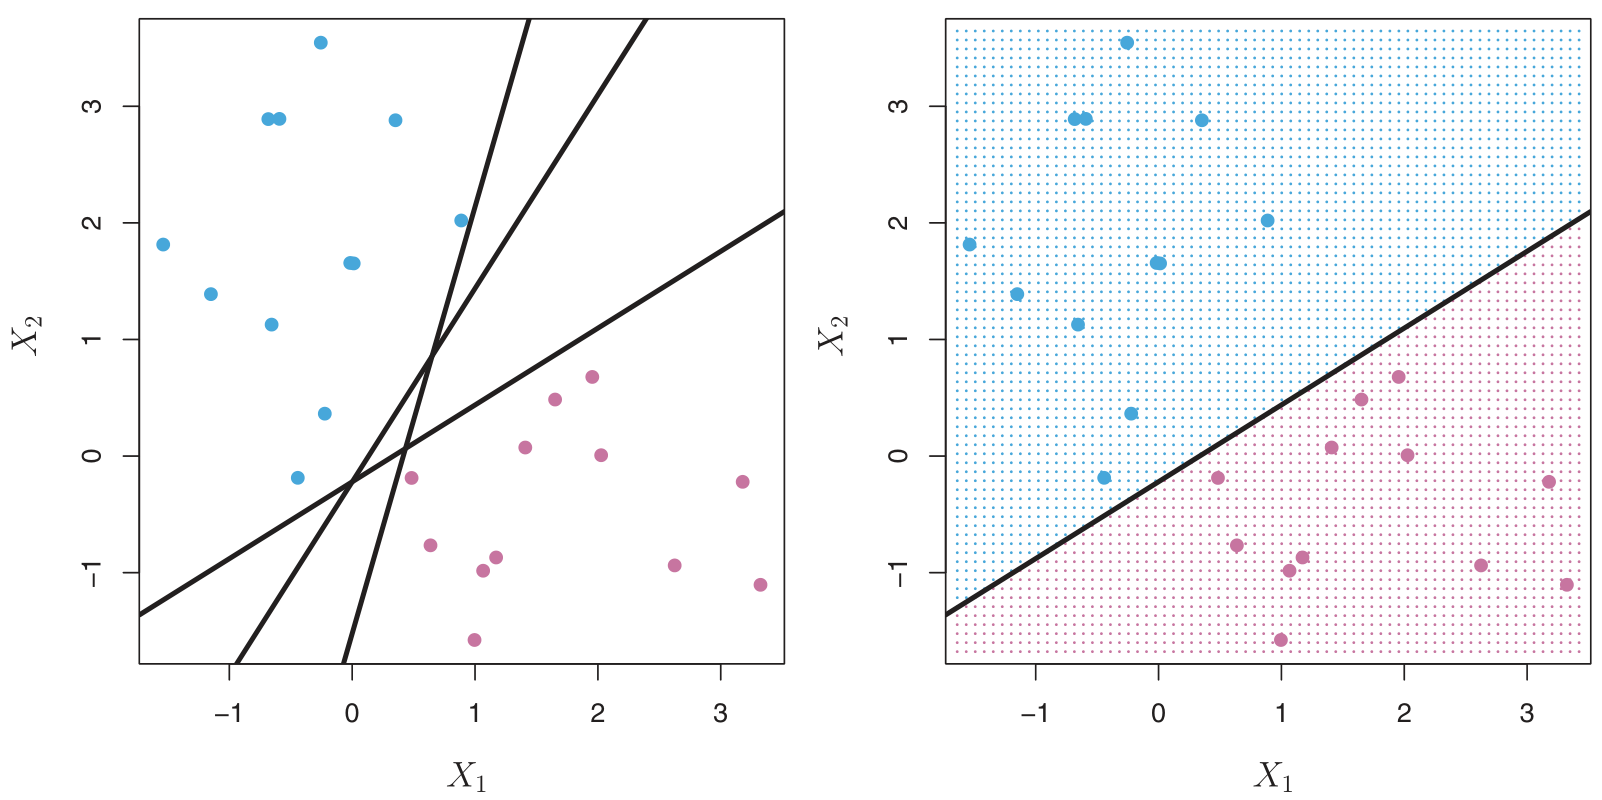
\includegraphics[scale=0.2]{images/hyperplane.png}
    \end{center}

    \textbf{Question}

    If our data can be perfectly separated using a hyperplane, then there will 
    be an infinite number of such hyperplanes. Which hyperplane would be the most 
    appropriate decision boundary?
\end{frame}





\begin{frame}
    \frametitle{Maximal Margin Classifier}
    \framesubtitle{Classification Using the Maximal Margin Classifier}
    \begin{block}{Margin}
        The minimal distance from observations to a given separating hyperplane.
    \end{block}

    \begin{block}{The Maximal Margin Hyperplane}
        The maximal margin hyperplane is the separating hyperplane 
        for which the margin is maximized.
    \end{block}

    \begin{block}{Support Vectors}
        Observations that are closest to the separating hyperplane are called support vectors.
    \end{block}
\end{frame}




\begin{frame}
    \frametitle{Maximal Margin Classifier}
    \framesubtitle{Construction of the Maximal Margin Classifier}
    We are now constructing the maximal margin hyperplane based on a set 
    of $n$ training observations $x_1, \cdots, x_n \in \mathbb{R}^p$ and 
    associated class labels $y_1, \cdots, y_n \in \{-1,1\}$. 
    \begin{gather*}
        \underset{\beta_0,\beta_1,\cdots,\beta_p}{\max} \quad M \quad \\
        \text{s.t.}
        \begin{cases}
            \sum_{j=1}^{p}\beta_j^2=1 \\
            y_i(\beta_0+\beta_1x_{i1}+\beta_2x_{i2}+\cdots+\beta_px_{ip})\geq M, \forall \space i=1,\cdots,n
        \end{cases}
    \end{gather*}
    Note:

    $\sum_{j=1}^{p}\beta_j^2=1$ is not really a constraint on the hyperplane. 
    However, with this constraint, we can easily show that the perpendicular 
    distance from the $i$th observation to the hyperplane is given by 
    \begin{align*}
        d&=\frac{y_i(\beta_0+\beta_1x_{i1}+\beta_2x_{i2}+\cdots+\beta_px_{ip})}{\sqrt{\sum_{j=1}^{p}\beta_j^2}} \\
        &=y_i(\beta_0+\beta_1x_{i1}+\beta_2x_{i2}+\cdots+\beta_px_{ip})
    \end{align*}
\end{frame}




\begin{frame}
    \frametitle{Maximal Margin Classifier}
    \framesubtitle{The Non-separable Case}
    In many cases, no separating hyperplane exists and there is no maximal 
    margin classifier. The optimization problem has no solution with $M>0$.
    \begin{center}
        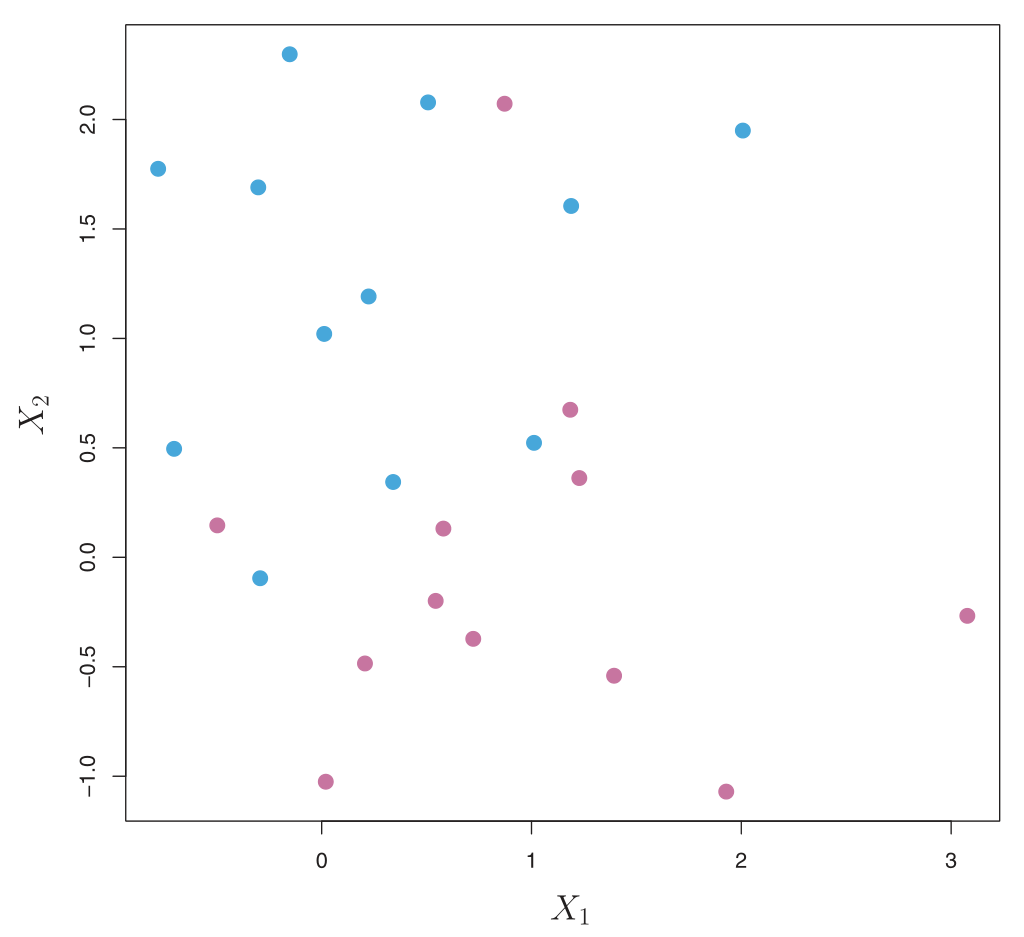
\includegraphics[scale=0.25]{images/nonseparable.png}
    \end{center}
\end{frame}



\begin{frame}
    \frametitle{Maximal Margin Classifier}
    The \textit{Maximal Margin Classifier} has some limitations:
    \begin{itemize}
        \item It is sensitive to outliers. 
        \item It is more likely to overfit the training data.
    \end{itemize}
\end{frame}

\begin{frame}
    \frametitle{Maximal Margin Classifier}  
    In order to solve the problems, sometimes it could be worthwhile to misclassify 
    a few training observations. 
    \begin{center}
        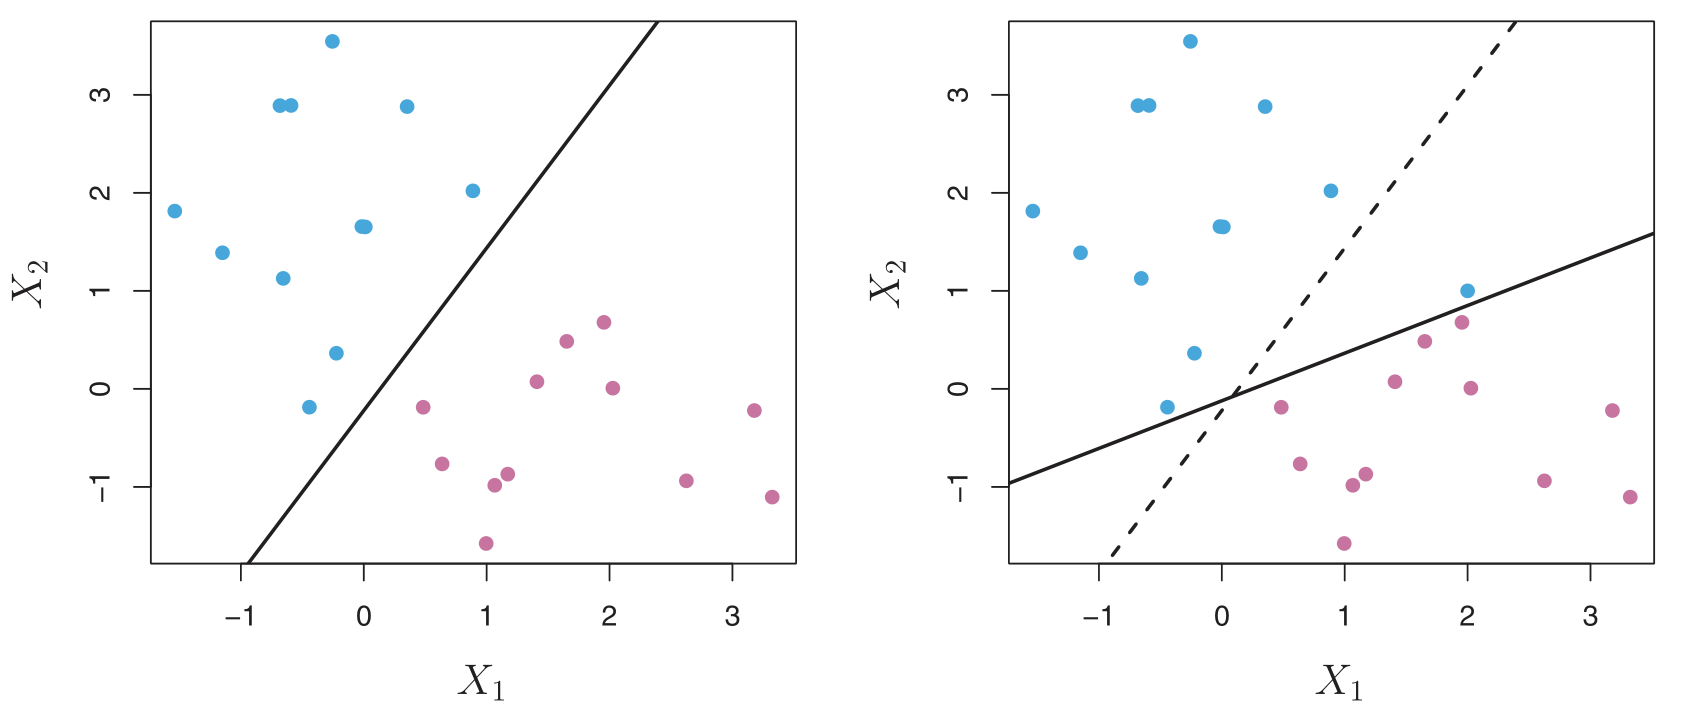
\includegraphics[scale=0.25]{images/outliers.png}
    \end{center}
\end{frame}

\begin{frame}
    \frametitle{Support Vector Classifiers}
    \framesubtitle{Overview of the Support Vector Classifier}
    \begin{block}{The Support Vector Classifier}
    The \textit{Support Vector Classifier} is a \textit{soft margin classifier} 
    that allows for some misclassified observations in order to improve 
    generalization ability.
    \end{block}

    The Support Vector Classifier ensures
    \begin{itemize}
        \item Greater robustness to individual observations
        \item Better classification of \textit{most} of the training observations
    \end{itemize}
\end{frame}

\begin{frame}
    \frametitle{Support Vector Classifiers}
    \framesubtitle{Classification Using the Support Vector Classifier}
    Support vector classifier comes down to an optimization problem
    \begin{gather*}
        \underset{\beta_0,\beta_1,\cdots,\beta_p,\epsilon_1,\cdots,\epsilon_n}{\max} 
        \quad M \quad \\
        \text{s.t.}
        \begin{cases}
            \sum_{j=1}^{p}\beta_j^2=1 \\
            y_i(\beta_0+\beta_1x_{i1}+\beta_2x_{i2}+\cdots+\beta_px_{ip})\geq M(1-\epsilon_i) \\
            \epsilon_i \geq 0, \sum_{i=1}^n\epsilon_i \leq C
        \end{cases}
    \end{gather*}

    \begin{itemize}
        \item $C$ is a nonnegative parameter
        \item $M$ is the width of the margin
        \item $\epsilon_1,\cdots, \epsilon_n$ are slack variables
    \end{itemize}
\end{frame}

\begin{frame}
    \frametitle{Support Vector Classifiers}
    \framesubtitle{Classification Using the Support Vector Classifier}
    \begin{block}{Nonnegative tuning parameter}
        $C$ bounds the sum of the $\epsilon_i$'s so it determines the number and severity of 
        the violations to the margin that we will tolerate. We can think of $C$ as a \textit{budegt} 
        for the amount that the margin can be violated by the $n$ observations.

        $C$ controls the bias-variance trade-off of the support vector classifier. 
        \begin{itemize}
            \item When $C$ is smaller, we seek narrow margins that are rarely violated. In this case, the classifier may overfit the data and have low bias and high variance.
            \item When $C$ is larger, the margin is wider and we allow more violations. In this case, the classifier may underfit the data and have high bias and low variance.
        \end{itemize}
    \end{block}
\end{frame}

\begin{frame}
    \frametitle{Support Vector Classifiers}
    \framesubtitle{Classification Using the Support Vector Classifier}
    \begin{center}
        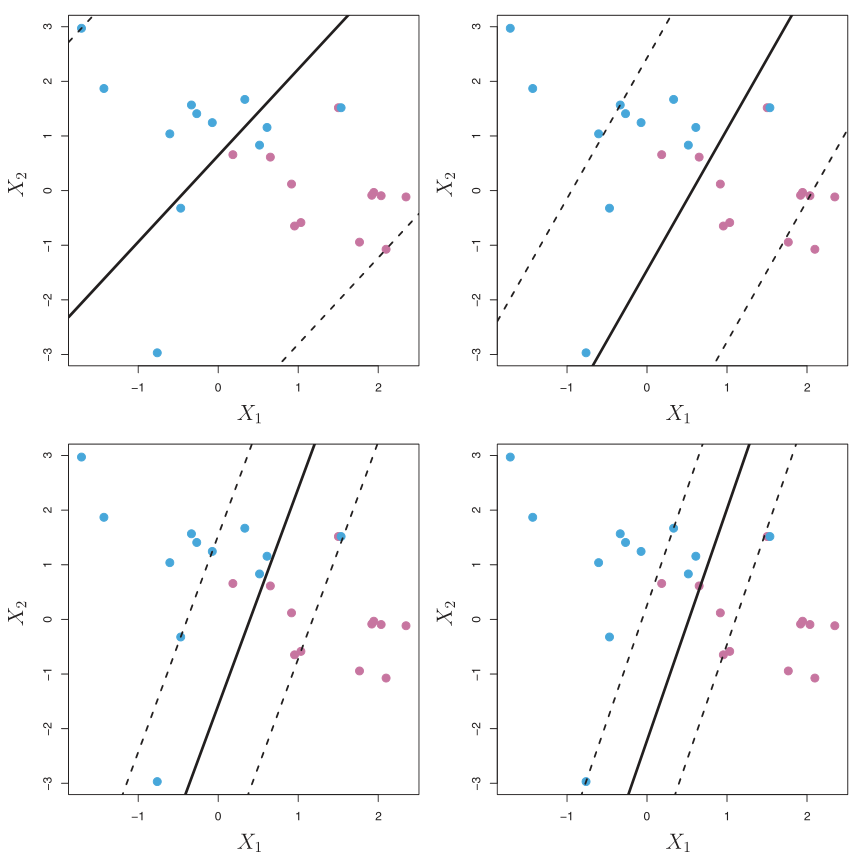
\includegraphics[scale=0.3]{images/C.png}
    \end{center}
\end{frame}

\begin{frame}
    \frametitle{Support Vector Machines}
    \framesubtitle{Classification with Non-linear Decision Boundaries}
    What if the data is non-linearly separable? The \textit{support vector classifier} 
    performs poorly in this setting.
    \begin{center}
        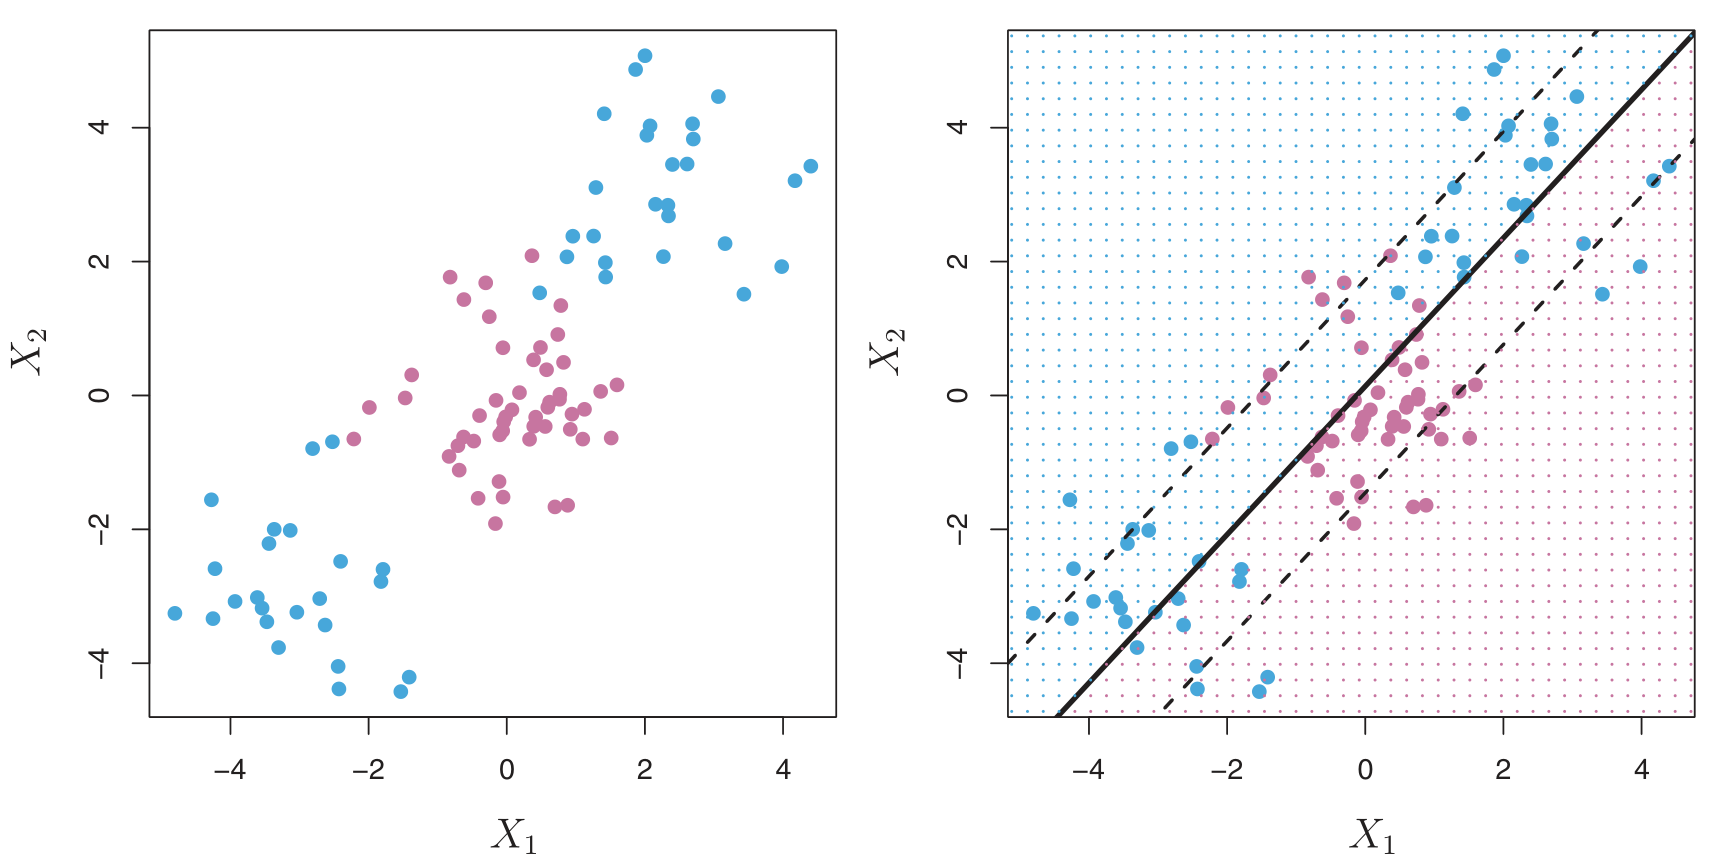
\includegraphics[scale=0.2]{images/non-linear.png}
    \end{center}
\end{frame}

\begin{frame}
    \frametitle{Support Vector Machines}
    \framesubtitle{Classification with Non-linear Decision Boundaries}
    Rather than fitting a support vector classifier using $p$ features, 
    we could instead fit a support vector classifier using $2p$ features
    \[X_1,X_1^2,X_2,X_2^2,\cdots,X_p,X_p^2 \] 
    Then the optimization problem would become
    \begin{gather*}
        \underset{\beta_0,\beta_{11},\beta_{12},\cdots,\beta_{p1},\beta_{p2},\epsilon_1,\cdots,\epsilon_n}
        {\max} \quad M \quad \\
        \text{s.t.}
        \begin{cases}
            \sum_{j=1}^p\sum_{k=1}^2\beta_{jk}^2=1 \\
            y_i(\beta_0+\sum_{j=1}^{p}\beta_{j1}x_{ij}+\sum_{j=1}^{p}\beta_{j2}x_{ij}^2)\geq M(1-\epsilon_i) \\
            \sum_{i=1}^{n}\epsilon_i\leq C, \epsilon_i \geq 0
        \end{cases}
    \end{gather*}
\end{frame}


\begin{frame}
    \frametitle{Support Vector Machines}
    \framesubtitle{Classification Using the Suport Vector Machine}
    \begin{block}{SVM}
        The \textit{support vector machine} (SVM) is an extension of 
        the support vector classifier that results from enlarging the 
        feature space in a specific way, using \textit{kernels}.
    \end{block}
    
    \begin{center}
        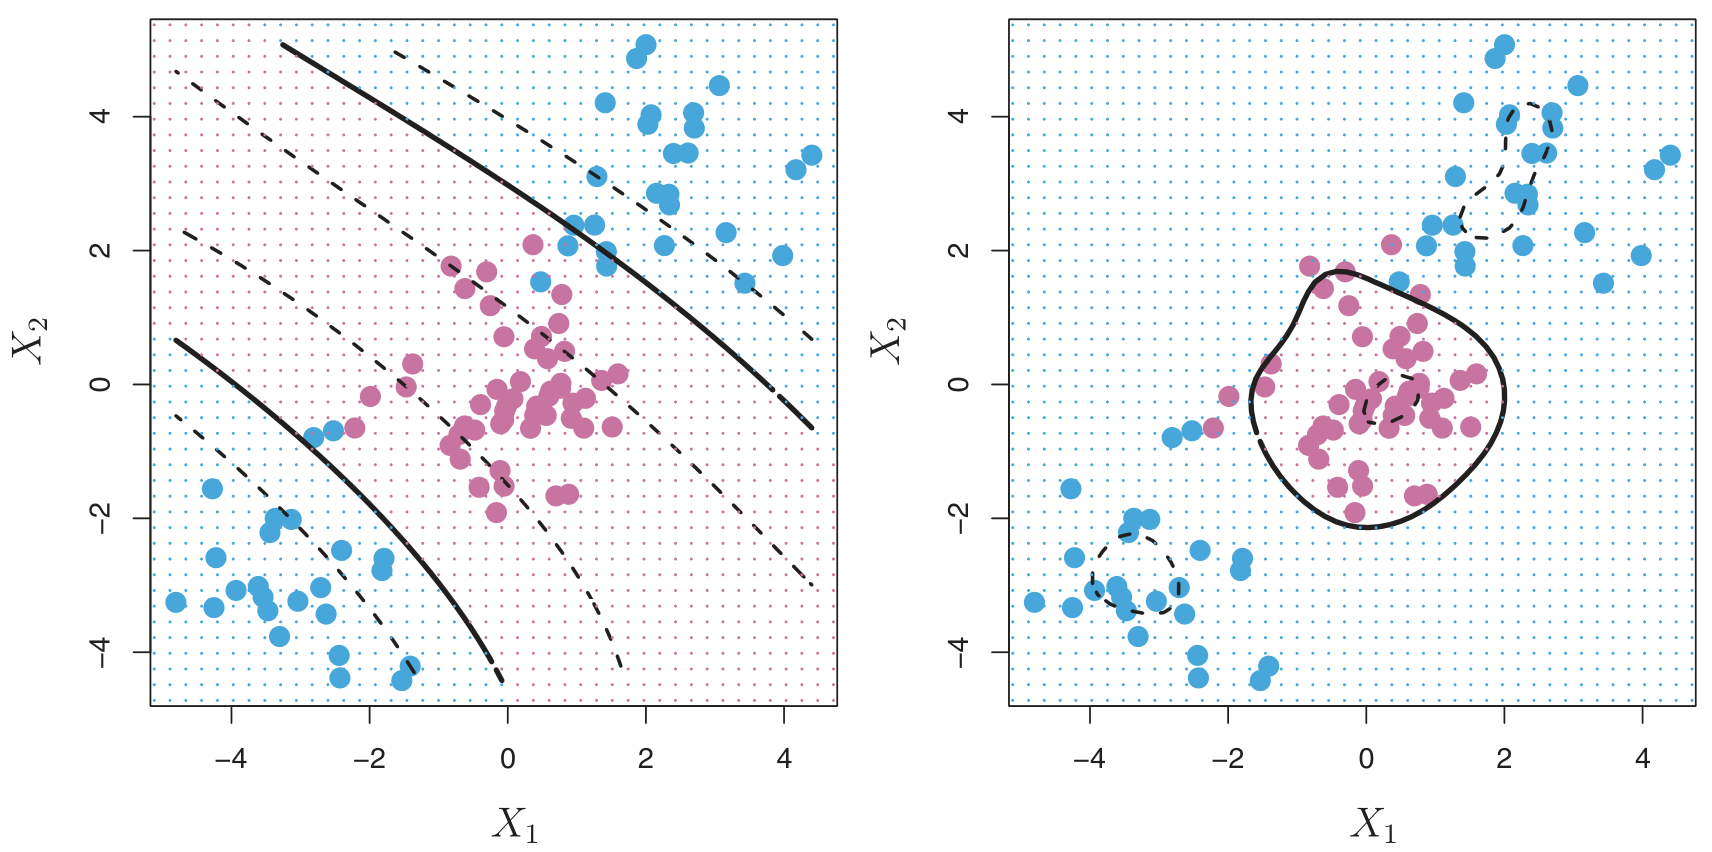
\includegraphics[scale=0.2]{images/kernel.png}
    \end{center}
\end{frame}



\begin{frame}
    \frametitle{Support Vector Machines}
    \framesubtitle{Classification Using the Suport Vector Machine}
    \textbf{Why are we interested in kernels?}
    \bigskip

    Our goal is to enlarge the feature space so that the data can be linearly separated. 
    Since the solution to the optimization problem only involves the \textit{inner product} of 
    the observations, we therefore want to find a more efficient way in computing the inner 
    product between each pair of data in the feature space or each pair of its expansion. 
    \textit{Kernels} are such functions that can give us the inner product of two inputs without even 
    knowing each input.
\end{frame}


\begin{frame}
    \frametitle{Support Vector Machines}
    \framesubtitle{Classification Using the Suport Vector Machine}
    \begin{block}{Kernel}
        A \textit{kernel} is a function that quantifies the similarity of two 
        observations.
        \[K(x_i,x_{i'}) \] 
        \begin{itemize}
            \item Linear kernel: $K(x_i,x_{i'})=\sum_{j=1}^{p}x_{ij}x_{i'j}$.
            \item Polynomial kernel: $K(x_i,x_{i'})=(1+\sum_{j=1}^{p}x_{ij}x_{i'j})^d$.
            \item Radial kernel: $K(x_i,x_{i'})=\exp(-\gamma\sum_{j=1}^p(x_{ij}-x_{i'j})^2)$
        \end{itemize}
    \end{block}
\end{frame}

%\begin{frame}
%\frametitle{Support Vector Machines}
%\begin{table}
%\begin{tabular}{r l}
%    \toprule
%    \textbf{Name} & \textbf{General idea} \\
%    Maximal Margin Classifier & 
%    \begin{itemize}
%        \item A hard margin classifier
%        \item No misclassification
%        \item Separable case
%    \end{itemize}\\
%    Support Vector Classifier &
%    \begin{itemize}
%        \item A soft margin classifier
%        \item Some misclassification 
%        \item Non-separable case
%    \end{itemize} \\
%    Support Vector Machine & 
%    \begin{itemize}
%        \item A soft margin classifier 
%    \end{itemize}
%    \bottomrule
%\end{tabular}

%\end{table}
%\end{frame}

\begin{frame}
    \frametitle{SVMs with More than Two Classes}
    \textbf{Question}

    The SVM can only deal with the binary classification. 
    What if we have multiple classes? How can we extend SVMs 
    to a more general setting?

    Two most popular approaches:
    \begin{itemize}
        \item One-Versus-One Classification
        \item One-Versus-All Classification
    \end{itemize}
\end{frame}

\begin{frame}
    \frametitle{SVMs with More than Two Classes}
    Suppose there are $K>2$ classes
    \begin{block}{One-Versus-One Classification}
        A \textit{one-versus-one} approach constructs $K \choose 2$ SVMs, 
        each of which compares a pair of classes.
        \begin{itemize}
            \item Training $\frac{K(K-1)}{2}$ classifiers.
            \item Each training procedure uses on average $\frac{2}{K}$ of the training data.
        \end{itemize}
    \end{block}

    \begin{block}{One-Versus-All Classification}
        A \textit{one-versus-all} approach constructs $K$ SVMs, each of which 
        compares one of the $K$ classes to the remaining $K-1$ classes.
        \begin{itemize}
            \item Training $K$ classifiers.
            \item Each training procedure uses the entire training data.
        \end{itemize}
    \end{block}
\end{frame}

\begin{frame}
    \frametitle{Reference}
    \footnotesize{
        \begin{thebibliography}{99}
            \bibitem[Springer, 2013]{p1} G. James, D. Witten, R. Tibshirani
            \newblock An Introduction to Statistical Learning with Application in R
            \newblock \emph{Support Vector Machines} 337-356
        \end{thebibliography}
    }
\end{frame}

\begin{frame}
    \Huge{\centerline{The End}}
\end{frame}

\end{document}

